\chapter{Difference-in-Differences with Spatial Spillovers}

% ------------------------------------------------------------------------------
\section{Introduction}
% ------------------------------------------------------------------------------

Empirical work in economics often considers settings where a policy targets units grouped by geographic boundaries but the effect of treatment spills over onto `nearby' units.\footnote{The framework of this paper applies to any setting with a well-defined measure of distance, e.g. geographic distance, economic distance such as supply chains, node distance in a graph, or social relationships in schools or cities.} For example, individuals in the surrounding area can travel across borders to receive treatment (e.g. a new  hospital serves nearby residents); or shocks to a labor market can affect nearby areas (e.g. a new factory increases service sector spending in the entire commuting zone). In these settings, a common approach involves using a structural model to account and control for general equilibrium effects. For example, trade models generate a market access term that effectively controls for such effects \citep{Donaldson_Hornbeck_2016}, or network models suggest a linear-in-means model controlling for the average characteristics of a unit's peers, e.g. proportion of peers treated \citep{manski1993identification,goldsmith2013social,Miguel_Kremer_2004}. 

However, researchers often wish to remain agnostic to structural assumptions, preferring minimal and transparent restrictions that, when made, allow for identification of treatment effects. This paper uses the potential outcomes framework proposed by \citet{vazquez2023identification} to consider non-parametric identification in difference-in-differences settings under the presence of spatial spillovers. In this framework, potential outcomes are now characterized by a unit's treatment status as well as the `exposure' to the treatment status of other units. Identification arguments are then made by imposing assumptions on the potential outcomes. 

Under the more general potential outcome framework, there are many potential treatment effects that can be formed. I consider identification of two relevant treatment effects that are common in the literature on interference \citep{savje2021average}. First, there is the `switching effect' which is the relevant parameter for local policymakers who want to answer, ``What is the effect of switching my treatment status, holding fixed all other units' treatment?''. I show that identification of the switching effect is a difficult problem which in a difference-in-differences framework would require the researcher to identify treated and control units that have the same level of exposure.\footnote{\citet{xu2023difference} takes this approach and discusses estimation and inference about this estimate.} 

The second effect of interest is the `total effect', which is the relevant parameter for national policymakers who want to answer, ``What is the average effect of implementing the entire treatment regime?''. This treatment effect is useful in post-hoc analyses analyzing the effect of implementing the observed treatment vector. This paper identifies simple and interpretable assumptions that allow for identification of the total effect. In settings where researchers are willing to impose an assumption that spillovers are `local', i.e. spillovers only impact units within a certain distance of treatment, I show the total effect can be identified with a parallel trends assumptions between treated and non-affected `far-away' units. The local spillovers assumption is reasonable in settings where travel is the primary driver of spillovers (e.g. people in nearby jurisdictions travel to the treated location). However, this assumption may not hold in the case of large general equilibrium shocks that affect units far away from the treatment area, such as when New York's economy impacts San Francisco.

In this framework, I evaluate common practices in empirical work. First, I show that the standard difference-in-differences estimator produces biased estimates for the total effect. This bias arises from the fact that untreated units that are "close" to treated units experience treatment effects, thereby failing to identify the counterfactual trend. The difference-in-differences estimate averages the spillover onto the "close" control units into the untreated units' change in outcomes. As a result, the spillover is subtracted from the estimated treatment effect, introducing bias in the opposite sign of the spillover effect. 

This problem is generally well understood, and it is common to either drop or include a dummy for nearby units in the standard two-way fixed effect model. This method consistently estimates the total effect under the assumptions I present in this paper. In this sense, this paper formalizes and clarifies the assumptions needed for this method. 

To show the importance of considering spillover effects and the utility of my estimators, I revisit analyses of place-based policies in urban economics in section \ref{sec:tva}. I revisit the analysis of the Tennessee Valley Authority by \citet{Kline_Moretti_2014a}. The Tennessee Valley Authority was a large-scale New Deal program that lowered the cost of power for industrial firms \citep{Kitchens_2014}. The scale of federal investment in the region was large and the pro-manufacturing benefits likely spread further than the Authority's boundary due to the electrification infrastructure and agglomeration economies \citep{severnini2023power}. I show that estimation by difference-in-differences fails to account for these spillovers and therefore the authors obtain biased estimates of the total effect of the Tennessee Valley Authority. For agriculture employment, I find that the long-run spillovers cause the original estimates to be about 40 percent too small for agriculture employment and 40 percent too large for manufacturing employment. 
% Following this empirical application, I briefly discuss how my framework fits into a larger discussion on identification strategies with place-based policies.
% (-0.0739 - -0.0514) / (-0.0514) = 43.7\% increase
% (0.0350 - 0.0560) / (0.0560) = 37.5\% decrease

Last, in section \ref{sec:event_study}, I extend estimation of treatment and spillover effects into settings with staggered-treatment timing by extending the work of \citet{Gardner_2021,Borusyak_Jaravel_Spiess_2021}.\footnote{I also briefly discuss how to adapt the estimation strategy of \citep{Callaway_SantAnna_2020}.} The proposed two-stage estimator first estimates unit and time fixed-effects using untreated/not-yet-treated observations. Since some control/not-yet-treated units can be affected by spillovers, these units must be removed to consistently estimate the unit and time fixed-effects. Then these estimated unit and time fixed-effects are subtracted from the observed outcome \textit{in the full sample}. The resulting differenced outcomes are then regressed on the treatment and spillover variables to estimate treatment and spillover effects. In the appendix, I demonstrate the method by revisiting the analysis by \citet{Bailey_Goodman_Bacon_2015} of Community Health Centers which provided low-cost primary care to impoverished areas.

This paper contributes to the literature that focuses on estimation of treatment effects with spatial spillovers using the difference-in-differences framework. Most work derives results for specific spillover mappings \citep{Clarke_2017,Berg_Streitz_2019,veribtsky2021causal,Delgado_Florax_2015}. My paper is the first to consider non-parametric identification in terms of general potential outcomes. My paper also advances the literature by considering estimation of treatment effects and spillover effects in settings with staggered-treatment timing. If I assume the particular functional forms for potential outcomes, I arrive at the same bias equation as theirs. \citet{xu2023difference} complements this paper well, focusing on identification and inference on the `switching effect'. 

This paper relates to a broad literature on spillover effect estimation in randomized experiments.\footnote{See \citet{sobel2006randomized} and \citet{Hudgens_Halloran_2008} for early work. See \citet{Hu_Li_Wager_2021}, \citet{savje2021average}, and \citet{vazquez2023identification} and references therein for recent work on this.} There are two main strands of this literature. First, there is a large literature on the estimation of treatment effects in the presence of spillovers using a `partial identification' framework where units are in distinct treatment clusters and outcomes depend on the treatment status within the observation's cluster only.\footnote{ \citet{Angelucci_DiMaro_2016} provides an overview of estimation of treatment effects in the presence of ``within-group'' spillovers. Empirical examples include \citet{Halloran_Struchiner_1995,sobel2006randomized,Miguel_Kremer_2004,Angrist_2014}.} Estimation compares units in the partially treated clusters with control units in completely untreated clusters which do not receive spillover effects. This allows standard difference-in-differences estimation of both the total effect (treatment effect on the treated) and spillover effects (treatment effect on the untreated in the treated clusters). However, my proposed estimator focuses on a setting without distinct clusters.

There is also a nascent literature exploring estimation of treatment and spillover effects which does not require a completely untreated cluster in experimental settings (\citet{savje2021average}; \citet{vazquez2023identification}; \citet{Hu_Li_Wager_2021}; \citet{yu2022estimating}). Those papers' identification results rely on \textit{design-based} assumptions around the treatment-assignment mechanism. Difference-in-differences, however, relies on \textit{model-based} assumptions on the potential outcomes (i.e. parallel-trends assumption) for identification in non-experimental settings. I contribute to this literature by formalizing identification results of different treatment effects in non-experimental settings. \citet{wang2020design} consider estimation of treatment effects in spatial settings under design-based settings and make a similar `local' spillovers assumption as this paper. 


% ------------------------------------------------------------------------------
\section{Theory}
% ------------------------------------------------------------------------------

There are a set of units $i \in \{1, \dots, N\}$ observed for periods $t \in \{0,1\}$ and treatment turns on between periods for some of the units. The framework is extended to staggered treatment adoption below. Let $D_i$ denote an indicator for unit $i$ being treated and the vector of treatment assignments as $\bm{D} = (D_1, \dots, D_n)'$. Since units can be impacted by the vector of treatment assignments, the general potential outcome notation is given by $Y_{it}(\bm{D})$. To simplify the high-dimensional set of potential outcomes, we follow \citet{aronow2017estimating,vazquez2023identification}, and introduce an `exposure mapping' which summarizes how a unit is exposed to spillovers: $h_i(\bm{D}): \{0, 1\}^N \to \mathcal{H}$ for some space $\mathcal{H}$ with $\dim(\mathcal{H}) \leq N$. For example, researchers might think $h_i(\bm{D})$ to be an indicator variable equal to one if any contiguous units are treated. The exposure mapping simplifies the potential outcome notation by imposing that if two treatment vectors $\bm{D}$ and $\tilde{\bm{D}}$ have $h_i(\bm{D}) = h_i(\tilde{\bm{D}})$, then the potential outcomes are also equal. Potential outcomes therefore can be written as $Y_{it}(D_i, h_i(\bm{D}))$. In the counterfactual world without treatment, we write the potential outcome as $Y_{it}(0, \bm{0})$ where $\bm{0} \in \mathcal{H}$ is defined as zero-exposure.

Often, researchers will try to parameterize potential outcomes, i.e. selecting a function $h_i(\cdot)$, by reasoning through the nature of the spillovers and subsequent estimation will rely on the functional form assumptions made by researchers. This paper will take an alternative approach to identification and estimation which will allow for estimation of treatment effects without requiring direct knowledge of the functional form of the exposure mapping/potential outcomes. 

Following \citet{Borusyak_Jaravel_Spiess_2021} and \citet{de2024difference}, our analysis views our panel and the treatment vector $\bm{D}$ (and hence exposure mappings) as fixed. Therefore, the uncertainty in the framework comes from stochastic potential outcomes.\footnote{See appendix section A.2 of \citet{Borusyak_Jaravel_Spiess_2021} for further discussion on fixed-design. \citet{xu2023difference} focuses on inference in a similar finite population setting.} In most of the related literature on interference, the treatment design and hence the distribution of exposure mappings is known (given $h$) so expectations can be taken without conditioning on the vector of exposure mappings.\footnote{See \citet{savje2021average} and \citet{pollmann2020causal} for discussion of estimation and inference when the treatment design is known.} The focus of this article is on difference-in-differences where identification comes from assumptions on the potential outcomes.

% ------------------------------------------------------------------------------
\subsection{Treatment and Spillover Effects}
% ------------------------------------------------------------------------------

In setups without spillovers, the treatment effect for an individual unit is well defined as $\tau_i \equiv Y_{i1}(1) - Y_{i1}(0)$. In the presence of spillovers, multiple treatment effects can be defined in this setting. This subsection will define commonly used estimands and discuss their interpretation. In the following sections, we will discuss identification strategies.

The natural analogue to the above treatment effect which I will label the `switching effect' is:
\[
  \tau_{i, switch}(\bm{h}) \equiv Y_{i1}(1, \bm{h}) - Y_{i1}(0, \bm{h}).
\] 
This is the effect of changing only unit $i$'s treatment status while keeping their exposure to spillovers constant at some value $\bm{h}$. This treatment effect is policy-relevant as it summarizes what would happen if a `local' policymakers decide to enact the policy for unit $i$ (implicitly keeping $\bm{h}$ constant).\footnote{This is what \citet{savje2021average} call the `assignment-conditional unit-level treatment effect'.} It is important to note that the switching effect can depend on the level of exposure. For instance, consider the construction of libraries in towns \citep{berkes2021knowledge}. The effect of a new library in a town that is far away from any other library (exposure of $\bm{0}$) is different than a town that is very close to a neighboring town's library (large $\bm{h}$), hence the dependence of $\tau_{i, switch}$ on $\bm{h}$. Since the size of the switching effect depends on a unit's exposure level, we will consider an average switching effect at each value of exposure, 
\[
  \tau_{\text{switch}}(\tilde{\bm{h}}) \equiv 
  \expec{Y_{i1}\big( 1, \tilde{\bm{h}} \big) - Y_{i1}\big( 0, \tilde{\bm{h}} \big)}{D_i = 1, h_i(\bm{D}) = \tilde{\bm{h}}}.
\]

The second policy-relevant parameter is the `total effect`: 
\[
  \tau_{i,\text{total}} \equiv Y_{i1}(1, h_i(\bm{D})) - Y_{i1}(0, \bm{0}).
\]
As opposed to the switching effect, which keeps exposure constant, the total effect looks at turning on treatment \textit{and} going from zero exposure to $h_i(\bm{D})$ simultaneously. This can be thought of as going from the world with a \textit{complete} absence of treatment, $\bm{0}$ to the current treatment vector $\bm{D}$. Individual effects can be averaged over treated units to the `total effect of treatment on the treated': 
\[
  \tau_{\text{total}} \equiv \expec{Y_{i1}(1, h_i(\bm{D})) - Y_{i1}(0, \bm{0}) \ \vert \ D_i = 1}.
\]
This treatment effect is helpful for `national' policymakers to evaluate what \textit{were} the effects of the entire vector of \textit{enacted policies}.\footnote{\citet{yu2022estimating} label the `total effect' to be $\expec{Y_{i1}(1, h_i(\bm{D})) - Y_{i1}(0, \bm{0})}$ where the average is over all units including control units. Identification of this effect relies on assumptions about experimental-design so this paper does not pursuit identification of this effect.} 

We formalize the `spillover effect' as the difference in potential outcomes between being exposed to the observed spillover exposure and not being exposed:
\[
  \tau_{i,\text{spill}}(d) \equiv Y_{i1}(d, h_i(\bm{D})) - Y_{i1}(d, \bm{0}).
\]
This effect can differ based on treatment status as the magnitude or even the causal mechanisms of spillovers might differ between treated and untreated units. For example, consider a targeted place-based policy that creates tax incentives to create businesses in designated census tracts. Nearby untreated census tracts could lose out on new business formation from this policy while nearby treated census tracts might benefit from agglomeration forces from a cluster of designated tracts. 

It is often also of interest to estimate the average spillover effects on subsets of units (e.g. all units experiencing non-zero exposure). Since it shows up in our below decomposition of the difference-in-differences estimand, we define the average spillover onto all the control units as
\[
  \tau_{\text{spill}}(0) = \expec{Y_{i1}(d, h_i(\bm{D})) - Y_{i1}(d, \bm{0})}{D_i = 0}.
\]
Estimation of spillover effects for different groups of units will be discussed in section \ref{sec:spill}.


% ------------------------------------------------------------------------------
\subsection{What Does Difference-in-Differences Estimate?}
% ------------------------------------------------------------------------------

With treatment effects properly defined, I will first derive what the standard difference-in-differences estimand identifies under a modified parallel trends assumption. 
\begin{assumption}[Parallel Counterfactual Trends]\label{assumption:parallel}
  Counterfactual trends do not depend on $D_i$:
  \[ 
    \expec{Y_{i1}(0, \bm{0}) - Y_{i0}(0, \bm{0}) \ \vert \ D_i = 1 } = 
    \expec{Y_{i1}(0, \bm{0}) - Y_{i0}(0, \bm{0}) \ \vert \ D_i = 0 }
  \]
\end{assumption}
This assumption states that in the absence of treatment and with zero exposure (not just the absence of individual $i$'s treatment), the change in potential outcomes from period 0 to 1 do not depend on treatment status. When the stable-unit treatment value assumption (SUTVA) is satisfied, all units have zero exposure and this assumption generalizes to the classic parallel counterfactual trends assumption. Second, I make the standard assumption `no anticipation' assumption that units do not adjust their actions in period $0$ from knowledge of future treatment:
\begin{assumption}[No Anticipation]\label{assumption:no-anticipation}
  $\expec{ Y_{i0}(D, \bm{h}(\bm{D})) } = \expec{ Y_{i0}(0, \bm{0}) }$.
\end{assumption}

With these assumptions, we derive what the standard difference-in-difference estimand identifies.
\begin{proposition}[Decomposition of Difference-in-Differences Estimand]\label{prop:bias}\ \\    
  If assumptions \ref{assumption:parallel} and \ref{assumption:no-anticipation}, the population difference-in-differences estimand can be decomposed as follows:
  \begin{align}\label{eq:did} 
      &\expec{Y_{i1} - Y_{i0}}{D_i = 1} - \expec{Y_{i1} - Y_{i0}}{D_i = 0}= \tau_{\text{total}} - \tau_{\text{spill}}(0)
  \end{align}
\end{proposition}
The proof is given in Appendix \ref{sec:spillover-proofs}, but the intuition is as follows. The change in outcomes among control units includes both the parallel counterfactual trend and the average spillover effect onto control units. Since $\hat{\tau}$ is found by subtracting the change in outcomes among the control units, we subtract the average spillover effect onto the control, $\tau_{\text{spill}}(0)$. 

% ------------------------------------------------------------------------------
\subsection{Identification of Treatment Effects}\label{sec:remove_bias}
% ------------------------------------------------------------------------------

% ------------------------------------------------------------------------------
\subsubsection{Switching Effect}
% ------------------------------------------------------------------------------

It is difficult to identify the switching effect in general as identifying the unobserved counterfactual outcome $Y_{i1}(0, h_i(\bm{D}))$ requires knowledge of which control units have the same level of exposure. The reason for this can be seen by rewriting this in terms of a difference-in-differences style estimand:
\begin{align*}
    \tau_{\text{switch}}(\tilde{\bm{h}}) &= \expec{Y_{i1}(1, \tilde{\bm{h}}) - Y_{i0}(0,\bm{0})}{D_i = 1, \bm{h}(\bm{D}) = \tilde{\bm{h}}} \\ 
    &\quad\quad - \expec{Y_{i1}(0, \tilde{\bm{h}}) - Y_{i0}(0,\bm{0})}{D_i = 1, \bm{h}(\bm{D}) = \tilde{\bm{h}} }.
\end{align*}
The first term is identified by the observed outcomes of the treated units. The second term would typically be estimated using the control units with exposure $\tilde{\bm{h}}$ under a parallel trend assumption. This is difficult as it requires knowledge of the unobserved exposure mapping to identify control units with $h_i(\bm{D}) = \tilde{\bm{h}}$. In related work, \citet{xu2023difference} take the approach of parameterizing the exposure mapping and discusses doubly-robust estimates of the switching effect.

Since spillover effects show up in the second term, estimation of the average switching effect requires an additional assumption that spillover effects on the control units be on average the same as the treated units. As an example, this assumption could fail if units that would receive the largest negative spillover effects select into treatment to avoid them. The problem of effects showing up in the above decomposition is similar to those highlighted by \citet{Callaway_Goodman-Bacon_SantAnna_2021} for difference-in-differences with continuous treatment. See their discussion on `strong parallel trends'

% \begin{assumption}[Switching Effect Parallel Trends]\label{assumption:parallel-switching}
%   For a given exposure, $\tilde{\bm{h}}$, counterfactual trends do not depend on $D$:
%   \[ 
%     \expec{Y_{i1}(0, \tilde{\bm{h}}) - Y_{i0}(0, \bm{0}) \ \vert \ D_i = 1, h_i(\bm{D}) = \tilde{\bm{h}} } = 
%     \expec{Y_{i1}(0, \tilde{\bm{h}}) - Y_{i0}(0, \bm{0}) \ \vert \ D_i = 0, h_i(\bm{D}) = \tilde{\bm{h}} }
%   \]
% \end{assumption}

% This assumption requires parallel trends among treated and control units at exposure $\tilde{\bm{h}}$. Under this assumption, the switching effect can be identified by a difference-in-differences estimand calculated using only units with an exposure of $\tilde{\bm{h}}$.

\begin{remark}
  Researchers may be tempted to introduce the parameterized exposure mapping interacted with a post dummy variable linearly in a two-way fixed effects model to ``compare individuals at the same level $\bm{h}$''. However, this assumes additive separability between the treatment dummy and the exposure mapping imposing homogeneity of switching effects for treated and untreated units. If the exposure mapping is continuous, then this also imposes switching effect grows linearly with $\bm{h}$. An alternative would be running difference-in-differences on subsets of treated and control units with the same value of $\bm{h}$. 
\end{remark}

% ------------------------------------------------------------------------------
\subsubsection{Total Effect}
% ------------------------------------------------------------------------------

To identify the total effect, additional assumptions on the nature of spillover effects are needed. In particular, I will formalize the idea that spillovers are `local' in that units are only affected by treatment if they are near treatment. For example, if treatment has to be accessed in person (e.g. access to abortion clinics), then it is natural that further away places are not affected by treatment. However, this assumption may fail under general equilibrium shocks that do not necessarily decay over distance. 

To formalize this assumption, let $d(i,j)$ be a function that measures the distance between units $i$ and $j$.\footnote{
  While the prose generally focuses on geographic distance, this could be any reasonable metric. For example, a measure of the connectedness between businesses where we assume larger values are more distant firms.
} 
For a given distance $\bar{d}$, let $S_{i}(\bar{d}) = \min_{j: \ D_j = 1} d(i,j) \leq \bar{d}$ be an indicator equal to one if unit $i$ is within $\bar{d}$ miles of the closest treated unit.
\begin{assumption}[Spillovers Are Local]\label{assumption:local}
  There exists a distance $\bar{d}$ such that 
  
  (i) For all units $i$,
  \[ 
      S_i(\bar{d}) = 0 \implies h_i(\bm{D}) = \bm{0}. 
  \]

  (ii) There exists treated and control units with $S_i(\bar{d}) = 0$.
\end{assumption}

Part (i) of assumption (\ref{assumption:local}) requires that spillovers are `local' in that units are no longer exposed to spillovers after some maximum distance $\bar{d}$. Part (ii) of Assumption (\ref{assumption:local}) requires that there exists control and treated units with no exposure. This assumption is far less strict than the identifying assumption for the switching effect in that we only need to identify which units have non-zero exposure and don't need to parameterize the exposure mapping any further.

The intuition behind identifying the total effect requires that we use control units experiencing no spillover effects to identify the counterfactual trend. However, this changes the necessary parallel trends assumption:
\begin{assumption}[Total Effect Parallel Trends]\label{assumption:parallel-mod}
  For a given $\bar{d}$, counterfactual trends are equal for the treated group and the far-away control group:
  $$
      \expec{Y_{i1}(0, \bm{0}) - Y_{i0}(0, \bm{0}) \ \vert \ D_i = 1}= 
      \expec{Y_{i1}(0, \bm{0}) - Y_{i0}(0, \bm{0}) \ \vert \ D_i = 0, S_i(\bar{d}) = 0}
  $$
\end{assumption}
With this assumption, we have the following identification result for the total effects:
\begin{proposition}[Identification of Total Effects]\label{prop:total_effect}
  Suppose that assumptions \ref{assumption:no-anticipation}, \ref{assumption:local}, and \ref{assumption:parallel-mod} hold. Then,
  \begin{equation}\label{eq:id_total}
    \tau_{\text{total}} = \expec{Y_{i1} - Y_{i0} \ \vert \ D_i = 1} - \expec{Y_{i1} - Y_{i0} \ \vert \ D_i = 0, S_i =0}.
  \end{equation}
\end{proposition}

Proofs are given in Appendix \ref{sec:spillover-proofs}. This proposition shows that if a researcher believes that spillover effects are `local', then estimation of the total effect on treated units only requires identifying which units are exposed to spillovers. The identifying assumption is that the control units are a valid comparison group \textit{after} removing the (potentially) exposed units. To estimate the total effect, we could replace the terms in proposition \ref{prop:total_effect} with their sample analogs.

\begin{remark}[Far-away control units and parallel trends]
  It is worth remarking on \nameref{assumption:parallel-mod} in terms of applied work. Often, researchers use only a subsample of observations that are close to treated observations. The idea is that if unobservable confounders evolve smoothly over space, then close units are more likely to be on similar counterfactual trends than units that are further away. The identification result and its corresponding estimator are formed by using further away units (i.e. units with $S_i = 0$). In this case, if parallel trends only hold for nearby control units, then focusing on further away units can fix the spillover bias but introduce bias from non-parallel trends. See appendix section \ref{sec:oz} for further discussion and an empirical example evaluating the 2017 U.S. Opportunity Zones using different identification strategies.
\end{remark}

\begin{remark}[Selection of $\bar{d}$]
  A natural question is why wouldn't researchers make the distance large to guarantee they have an unbiased estimate of $\tau_{\text{total}}$? Equation (\ref{eq:id_total}) should make this problem clear. Since these estimates rely on averages among units with $S_i = 0$, as $\bar{d}$ increases, the number of units with $S_i = 0$ decreases which yields more variable estimates. On the other hand, having units that experience spillovers not included in the $S_i$ indicator will leave some bias in the estimate.\footnote{Although, spillover effects typically will grow weaker over distance and if distant units are mistakenly treated as if they have zero exposure, bias should be small.} Therefore there is a bias-variance trade-off in extending the extent of $S_i$ that should be balanced by researchers guided by their particular economic context. Additionally, each value of $\bar{d}$ corresponds to a different effective control group and hence a different parallel trends assumption, rendering comparisons across $\bar{d}$ uninformative.
\end{remark}


\subsubsection{Spillover Effects}\label{sec:spill}

This section turns to identification of averages of spillover effects. To do so, it is typical to compare nearby control units to further away units. This  requires an additional parallel trends assumption that the far-away control units and the nearby control units are on the same trends:
\begin{assumption}[Spillover Effect Parallel Trends]\label{assumption:parallel-spill}
  For a given $\bar{d}$, we have: 
  \begin{align*}
    \expec{Y_{i1}(0, \bm{0}) - Y_{i0}(0, \bm{0}) \ \vert \ D_i = 0, S_i(\bar{d}) = 1} = 
    \expec{Y_{i1}(0, \bm{0}) - Y_{i0}(0, \bm{0}) \ \vert \ D_i = 0, S_i(\bar{d}) = 0}.
  \end{align*}
\end{assumption}

In this case, comparing control units with $S_i(\bar{d}) = 1$ to far-away control units will identify the average spillover effect on control units with $S_i(\bar{d}) = 1$:
$$
\expec{ Y_{i1}(d, h_i(\bm{D})) - Y_{i1}(d, \bm{0}) }{ S_i(\bar{d}) = 1, D_i = 0}
$$

Joint estimation of the total effect on the treated and the spillover effect on the nearby control units can be done using the following regression specification on the full sample:
\begin{equation}\label{eq:twfe_spill}
  Y_{it} = \tau D_i \one_{t = 1} + \gamma_0 (1 - D_i) S_i(\bar{d}) \one_{t = 1} + \mu_i + \lambda_t + \varepsilon_{it}.
\end{equation}

Note that since some units with $S_i(\bar{d}) = 1$ may not have positive exposure ($\bm{h}_i(\vec{D}) = \bm{0}$), this is not the average spillover effect for units with non-zero exposure. For example, if only units really close to treatment receive spillover effects and $S_i(\bar{d})$ contains a lot of units that experience no spillover effects, then $\hat{\tau}_{\text{spill, control}}$ could be estimated near zero even though some units experience substantial spillover effects. For example, reanalysis of \citet{linden2008estimates} in \citet{butts2023jue} finds that the arrival of sex offenders to a neighborhood has large impacts on homes within $0.05$ miles and much smaller impacts for homes between $0.05$ and $0.10$ miles. Selecting $\bar{d}$ to be $0.1$ estimated an effect that was about half as large as the estimated impact on the very close homes.

To better understand how spillover effects vary over distances, applied researchers will sometimes split up $S_i(\bar{d})$ into a set of $J$ concentric `rings' (e.g 0-20 miles, 20-40 miles, and 40-60 miles from the nearest treated unit). Equation (\ref{eq:twfe_spill}) can be modified as 
\begin{equation}\label{eq:twfe_rings}    
  y_{it} = \tau D_i \one_{t = 1} + \sum_{j=1}^J \gamma_j (1 - D_i) \text{Ring}_i^j \one_{t = 1}  + \mu_i + \lambda_t + \varepsilon_{it},
\end{equation}
where $\text{Ring}_i^j$ is an indicator for a control unit $i$ being in ring $j$ with $\sum_j \text{Ring}_{i}^j = S_i(\bar{d})$. The estimate $\hat{\tau}$ is still consistent for the total effect since the effective control group remains the same. However, interpretation of each $\hat{\gamma}_j$ as causal requires a yet stronger parallel trends assumption. Namely, units in each ring $j$ must be on the same parallel counterfactual trend as the $S_i(\bar{d}) = 0$ control group. If only assumption \ref{assumption:parallel-spill} is assumed, it is not possible separate variation in spillover effects from variation in counterfactual trends across rings. \citet{butts2023jue} shows that in some settings where you are willing to assume that parallel trends holds for all distances from treatment, a non-parametric estimator is available for average spillover effects as a function of distance. This assumption is more likely in very local settings where units do not vary in terms of temporal shocks.

% ------------------------------------------------------------------------------
\section{Applications in Place-Based Policy Analysis}
% ------------------------------------------------------------------------------

More generally, my framework provides important insights into identification strategies when analyzing the effects of place-based policies. There are two ways I contribute. First, \citet{Baum-Snow_Ferreira_2015} recognize the problem of spatial spillovers causing problems in identification and point to aggregation of units as a way to alleviate the problem (e.g. aggregating census tracts to metropolitan areas). However, this approach combines the treatment and spillover effects, which might each be of interest, into a singular aggregate effect. This method averages over heterogeneous effects (in magnitude or in nature) that might be of independent interest. The methods propose in this paper provide a strategy for disentangling treatment effect estimates with non-aggregated data. Subsection \ref{sec:tva} will revisit the analysis of a large-scale targeted policy on regional development. In this setting, spillover effects on nearby counties, via lost jobs, are of a very different nature than the direct impact on the targeted region and hence separate estimation if of practical interest. 

Second, my framework provides insight into different identification strategies often used in the literature. Since place-based policies are targeted to specific distressed areas, comparison units are often hard to find. Researchers have developed many identification strategies to find comparison units that are similar in terms of unobservables. First, researchers use border discontinuities to compare treated units to units just on the other side of the border. Other times, researchers compare approved applicants to narrowly rejected applicants. Both strategies aim to balance unobservables between treated and control units. A key difference in these identification strategies is the distance comparison units are from the treated area and therefore the former is more prone to bias due to spillovers than the latter. Subsection \ref{sec:oz} tries to highlight the differences in these identification strategies in the context of the U.S. Opportunity Zones created in 2017.

% ------------------------------------------------------------------------------
\subsection{The Tennessee Valley Authority}\label{sec:tva}
% ------------------------------------------------------------------------------

To illustrate the importance of accounting for spatial spillovers in the estimation of treatment effects, I revisit the analysis of the Tennessee Valley Authority (TVA) in \citet{Kline_Moretti_2014a}. The TVA program was a large-scale federal investment started in 1934 that focused on the construction of dams and transportation canals in an attempt to modernize the Tennessee Valley's economy. By the end of WWII, the TVA became the largest single power supplier in the country and significantly lowered the cost of wholesale energy for manufacturers.\footnote{More details on the program are found in \citet{Kline_Moretti_2014a}. The effects on wholesale electricity are discussed in \citet{Kitchens_2014}.} With over \$20 Billion (in 2000 dollars) spent which is hundreds of dollars transferred per person in the Authority, the impacts are very likely to extend past the authority's borders. \citet{Kline_Moretti_2014a} analyze a range of outcome variables, but I focus on agricultural and manufacturing employment. 
% Since the TVA primarily improved manufacturing industries through large-scale electrification, the authors predict that employment will grow in manufacturing and shrink in agricultural as workers switch to higher-paying manufacturing jobs. 

The analysis in \citet{Kline_Moretti_2014a} begins by comparing changes in county-level outcomes from 1940 to either 1960 (short run effects) or 2000 (long run effects) between treated counties in the Authority and control counties outside. The primary specification is
\begin{equation}\label{eq:tva}
    y_{c, t} - y_{c, 1940} = \alpha + \text{TVA}_c \tau + X_{c, 1940} \beta + (\varepsilon_{c, t} - \varepsilon_{c, 1940}),
\end{equation}
where $c$ denotes county, $\text{TVA}_c$ is an indicator variable for being in the Authority, and $y$ is a set of outcome variables (in logs).\footnote{The two-period difference-in-differences regression is equivalent to a first-difference regression. The authors use an Oaxaca-Blinder estimator on the first differences and the results of \citet{Kline_2011} show that this estimator is equivalent to a weighted difference-in-differences estimate. Their estimator does not differ much from the standard difference-in-differences results since the weights are not that different from uniform weights.} Pre-treatment control variables, $X_{c,1940}$, are included to allow for places to be on different long-term trends.\footnote{See footnote 8 in \citet{Kline_Moretti_2014a} for a full listing of control variables.} To improve the likelihood of the parallel trends assumption, they run a logistic regression to predict being in the TVA based on their set of control variables $X_{c,1940}$ and keep only observations in the top 75\% of predicted probability. The subsample produced from this exercise is presented in Figure \ref{fig:tva_sample}. 

In the paper, the authors discuss the nature of spillovers that they think can occur. For agriculture employment, the authors argue that improved wages in the TVA will draw agriculture workers out of nearby counties producing negative spillovers. For manufacturing, there are two countervailing forces \citep{Cuberes_Desmet_Rappaport_2021}. Positive spillovers from `urban access' would occur if electrification brought cheap power and agglomeration economies to the neighboring areas. The countervailing `urban shadow' would cause negative spillovers if firms chose to locate in the Authority that would have, in the absence of the program, decided to locate in nearby counties. My methodology will allow me to empirically test for these two forces in the data over time while removing their bias from the total effect estimates. 

\citet{Kline_Moretti_2014a} estimate (\ref{eq:tva}) to identify what I am calling the `total effect on the treated'. However, their point estimates compare, in part, changes in outcomes in TVA counties with changes in outcomes for neighboring counties that likely were impacted by the large-scale program. The authors do recognize the problem of spillover effects and the majority of the paper uses structural models to estimate the general equilibrium effects of the TVA. In this light, the re-analysis here is complementary to their work. 

% Figure: TVA Effective Sample and Spillover Variables
\begin{figure}[tb!]
    \caption{TVA Effective Sample and Spillover Variables}
    \label{fig:tva_sample}

    {\centering
        \resizebox{\textwidth}{!}{
            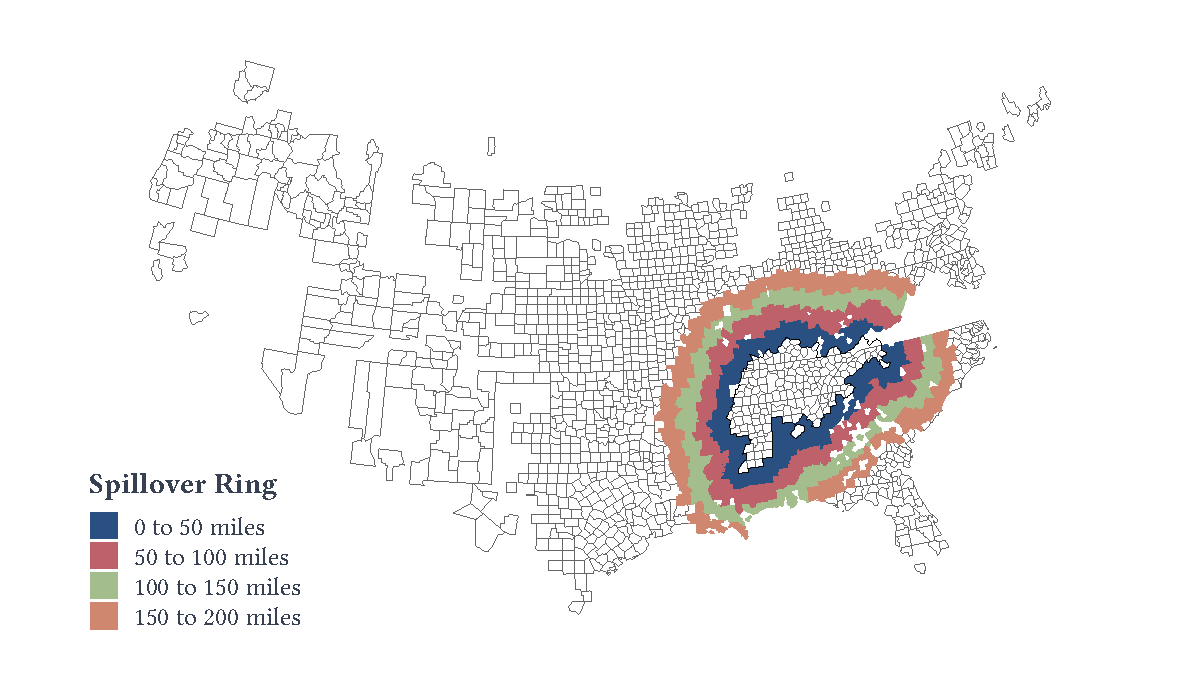
\includegraphics{figures/spatial-spillovers/tva/tva-sample.pdf}
        } 
    }
    {\footnotesize \textit{Notes:} The above figure plots all the counties used in the estimation. Counties that fall within the distance intervals $\{ (0, 50], (50, 100], (100, 150], (150, 200] \}$ measured in miles are colored by their respective bin.} 
\end{figure}

I extend their analysis to control for spatial spillovers in the difference-in-differences specification. To parameterize the exposure mapping, I use a set of rings as described in section \ref{sec:spill}. Specifically, 
the specification with spillovers is given as follows:  
\begin{equation}\label{eq:tva_spillover}
    y_{i, t} - y_{i, 1940} = \alpha + \text{TVA}_i \tau + \sum_{j \in \text{Dist}} \text{Ring}_i^j \gamma_j + X_{i, 1940} \beta + (\varepsilon_{i, t} - \varepsilon_{i, 1940}),
\end{equation} 
where $\text{Dist} = \{(0, 50], (50, 100], (100, 150], (150, 200]\}$ measured in miles and define $\text{Ring}_i^j$ as an indicator for being within the interval $d \in \text{Dist}$ away from the Authority and $t \in \{1960, 2000\}$. Figure \ref{fig:tva_sample} displays the four spillover variables by filling in each distance bin in a different color. The coefficients $\gamma_j$ estimate the average spillover effect onto control units for each of these distance bins. It's important to note that estimation of (\ref{eq:tva_spillover}) changes the comparison group to counties further away than 200 miles from the TVA.

The results of the long run analysis from 1940 to 2000 are presented in Panel A of Table \ref{tab:tva}. Each row contains the results for a different outcome variable (measured in logs). Columns (1)-(5) contain point estimates for $\tau$ and $\gamma_j$'s in different specifications. The point estimates can be interpreted as decadal growth rates in outcomes. The column labeled difference-in-differences estimates equation (\ref{eq:tva}). This estimate finds a decline in agricultural employment of about $5.1\%$ per decade and an increase in manufacturing employment of about $5.6\%$ per decade. 

% Table: Effects of Tennessee Valley Authority on Decadal Growth
\begin{table}[!tb]
  \caption{Effects of Tennessee Valley Authority on Decadal Growth}
  \label{tab:tva}
  \renewcommand{\arraystretch}{1.1}

  \begin{adjustbox}{width = \textwidth, center}
    \begin{tabular}{@{} l c@{\extracolsep{20pt}}c@{\extracolsep{4pt}}cccc @{}}
      % Head
      \toprule

      & \multicolumn{1}{c}{\textbf{Diff-in-Diff}} & \multicolumn{5}{c}{\textbf{Diff-in-Diff with Spillovers}} \\ 
      \cmidrule{2-2} \cmidrule{3-7}
      & & & TVA between & TVA between & TVA between & TVA between \\ 
      & TVA & TVA & 0-50 mi. & 50-100 mi. & 100-150 mi. & 150-200 mi. \\ 
      \textit{Dependent Var.} & (1) & (2) & (3) & (4) & (5) & (6) \\

      % Body
      \toprule
      \multicolumn{7}{l}{\textbf{Panel A:} 1940-2000} \\
      \midrule
      Agricultural employment   & $-0.0514^{***}$ & $-0.0739^{***}$ & $-0.0371^{**}$  &    $-0.0164$    & $-0.0298^{***}$ &  $-0.0157^{*}$ \\
                          &   $(0.0135)$    &   $(0.0163)$    &   $(0.0149)$    &   $(0.0114)$    &   $(0.0104)$    &   $(0.0095)$   \\
Manufacturing employment  & $0.0560^{***}$  &    $0.0350$     &    $-0.0203$    &    $-0.0245$    &    $-0.0331$    &  $-0.0296^{*}$ \\
                          &   $(0.0196)$    &   $(0.0267)$    &   $(0.0274)$    &   $(0.0338)$    &   $(0.0227)$    &   $(0.0166)$   \\


      \toprule
      \multicolumn{7}{l}{\textbf{Panel B:} 1940-1960} \\
      \midrule 
      Agricultural employment   & $0.0940^{***}$  &  $0.0856^{*}$   &    $-0.0062$    &    $-0.0042$    &    $-0.0303$    &    $-0.0039$   \\
                          &   $(0.0309)$    &   $(0.0473)$    &   $(0.0507)$    &   $(0.0487)$    &   $(0.0471)$    &   $(0.0339)$   \\
Manufacturing employment  &  $0.0894^{**}$  &  $0.0993^{**}$  &    $0.0228$     &    $0.0225$     &    $-0.0055$    &    $-0.0066$   \\
                          &   $(0.0348)$    &   $(0.0473)$    &   $(0.0554)$    &   $(0.0630)$    &   $(0.0399)$    &   $(0.0292)$   \\


      \bottomrule
    \end{tabular}
  \end{adjustbox}

  \note{
    Each row corresponds to an outcome variable. Each cell is the point estimate and the standard error for the variable described in the column title. All standard errors are Conley standard errors with a correlation cutoff of 200 miles following \citet{Conley_1999}. The column labeled `Diff-in-Diff' estimates (\ref{eq:tva}) by OLS and is similar to the estimate reported in \citet{Kline_Moretti_2014a}. The final four columns labeled `Diff-in-Diff with Spillovers' are estimates from (\ref{eq:tva_spillover}). $^{*} p< 0.1$; $^{**} p < 0.05$; $^{***} p < 0.01$.
  }

\end{table}

Turning to specification (\ref{eq:tva_spillover}) which includes spillovers, column (2) contains a point estimate for $\tau$ and columns (3)-(6) contain point estimates of the spillover effects $\gamma_j$. For agricultural employment, the point estimates show there was a decline in agriculture employment in control units near the Authority. For control units between 0 and 50 miles, column (4) indicates a decline in agricultural employment of $3.7\%$ per decade. Between 50 and 100 miles the point estimate is $-1.6\%$ per decade, between 100 and 150 miles the point estimate is $-3\%$ per decade, and between 150 and 2000 miles the point estimate is $-1.6\%$ per decade. This is likely because higher-paying manufacturing jobs within the Authority drew farm-worker migrants from nearby counties. Because the spillovers onto the control counties are negative, the original difference-in-differences estimator was positively biased. The new point estimate indicates a decline of agricultural employment of about $7.4\%$ per decade compared to $5.1\%$ in the standard difference-in-difference specification. 

For manufacturing, our point estimates for spillovers are consistently negative though imprecisely estimated. The spillover estimates suggest that neighboring counties potentially experienced negative spillover effects in the long run. Since there are negative spillover effects present, the new point estimate in column (2) of $3.5\%$ is smaller than the original estimate of $5.6\%$. The spillover estimates are evidence that in the long run, `urban shadow' (stealing manufacturing firms) forces dominate the benefits of `urban access' (agglomeration effects). 

To see how spillover effects from a large-scale place-based policy develop over time, Panel B in Table \ref{tab:tva} presents results for the effects of the Tennessee Valley in the short run using outcome data in 1960. Unlike in the long run, areas near the Tennessee Valley did not experience significant declines in agricultural employment in the short run. Since our long run analysis finds significant increases in high-paying manufacturing employment in the Tennessee Valley, this result is consistent with long run migration costs being lower than short run costs.

For manufacturing, there are potentially positive increases in manufacturing employment within 100 miles of the Tennessee Valley Authority and near-zero effects between 100 and 200 miles. In the short run, it appears that the effects of urban access and the cheap wholesale electricity dominated the effects of urban shadow. The effect of urban shadows can potentially be smaller in the short run if operating firms are unlikely to relocate. long run effects can be larger as entrant firms change their location decision and operating firms are slowly replaced which is what the long run spillover effect estimates suggest.

These results show that including spillovers in the estimation of treatment effects is potentially important and can lead to \textit{significant} differences in treatment effect estimates. Analysis of place-based policies that do not account for the fact that treatment effects can spill beyond the borders of treated areas can potentially be biased. More, the results suggest that the spillover effects caused by place-based policies change over time as frictions can create delays in re-optimizing behavior. 


% ------------------------------------------------------------------------------
\subsection{United States Opportunity Zones}\label{sec:oz}
% ------------------------------------------------------------------------------

In this subsection, I revisit the analysis of \citet{chen2023jue} on the 2017 Opportunity Zone program which created tax incentives for capital investment in targeted Census Tracts.\footnote{Concurrent work by \citet{Arefeva_2021} also estimates spillover to nearby opportunity zones using a different dataset and finds positive spillover effects on nearby census tracts as well.} The impacts of these kinds of programs is contentious in the literature. For example, there are a set of conflicting results on the impacts of the Empowerment Zones in the late 1990s with some papers suggesting that the Empowerment Zones reduced poverty rates while others finding near-zero effects.\footnote{See Table 1 of \citet{Neumark_Young_2019} for a summary of the various treatment effect estimates in the literature. \citet{Busso_Gregory_Kline_2013} compare census tracts in Empowerment Zones to census tracts that qualified and were rejected from the program. The rejected tracts are not typically geographically near accepted Empowerment Zones and they find large significant reductions in poverty rates. Meanwhile, \citet{Neumark_Kolko_2010} compare census tracts in Empowerment Zones to census tracts within 1,000 feet of the Zone. These control counties are likely the ones that experience the largest spillover effects and they find near-zero effects on poverty. My paper suggests that the former is the preferred strategy in the presence of significant spillovers onto nearby control units.} The analysis of the 2017 Opportunity Zones creates a nice setting to consider the differences between the strategies since which tracts were eligible but ultimately were not selected is public information.

To measure the affects of the opportunity zone program on housing prices, the authors collect a panel of census tracts with a measure of housing prices from the Federal Housing Finance Agency (FHFA) from 2014-2019.\footnote{The index tries to create a consistent price index that captures for changes in the composition of homes that are sold over time.} They produce estimates using two different identification strategies. First, they compare census tracts that were selected as Opportunity Zones to eligible, but ultimately not selected, census tracts. This estimation strategy relies on the assumption that since these census tracts are similar in nature to the treated census tracts (both meeting the program's criteria), it is likely that home prices would continue on similar trajectories in the absence of the program. The authors run a standard two-way fixed effect specification on the subsample of eligible census tracts:
\begin{equation}\label{eq:oz-eligible}
  Y_{it} = \mu_i + \mu_t + \tau d_{it} + \varepsilon_{it},
\end{equation}
where $Y_{it}$ is the annual change in the home price index, $\mu_i$ are tract fixed-effects, $\mu_t$ are time fixed effects, and $d_{it}$ is an indicator for treatment. 

The second identification strategy relies on comparing selected census tracts to geographically neighboring census tracts. This estimation strategy relies on the assumption that proximity of census tracts would face similar economic shocks and hence home prices would likely evolve in parallel. For each treated census tract, they find the nearest non-treated census tract to form a pair, $(i, \tilde{i}) \equiv \nu$. They then estimate the following equation:
\begin{equation}\label{eq:oz-neighbor}
  Y_{it} - Y_{\tilde{i}t}  = \mu_\nu + \tau d_{it} + u_{it},
\end{equation}
where $Y_{it}$ is the annual change in the home price index, $\mu_\nu$ are pair fixed-effects and $d_{it}$ is an indicator for treatment. 

A valid concern is that not-selected tracts were not selected because they were viewed as having better economic prospects than selected tracts, implying that a parallel trends assumption like in \ref{assumption:parallel-mod} is unlikely to hold. The authors provide evidence of parallel `pre-trends' for both the nearby tracts and the eligible but not-selected tracts, alleviating concerns in this context. The results of both estimation strategies are shown in Table \ref{tab:oz}. Column (1) and (2) show the results of estimating Equation (\ref{eq:oz-eligible}) and (\ref{eq:oz-neighbor}) respectively. The `not-selected' estimate finds a marginally significant effect of an increase in home prices of about 0.3\% annually while the `neighboring' estimate finds a strongly significant effect twice as large of about 0.65\%.\footnote{The authors use this estimate to rule out effects larger than $\approx 0.65 + 2 * 0.25 = 1.15\%$. As shown before, these estimates are biased upwards and hence the upper bound of effect size can be lowered to about $\approx 0.65\%$.} 

% Table: Effects of Opportunity Zones on Annual Home Price Growth
\begin{table}[!tb]
  \caption{Effects of Opportunity Zones on Annual Home Price Growth}
  \label{tab:oz}
  \renewcommand{\arraystretch}{1.1}

  \begin{center}
  \begin{tabular}{@{} l ccc @{}}
    % Head
    \toprule
    & (1) & (2) & (3) \\

    % Body
    \midrule
    Treat $\times$ Post     & 0.3033$^{*}$    & 0.6478$^{***}$              & 0.1788\\   
& (0.1661)        & (0.2457)                    & (0.1692)\\   
$<$ 1/2mi. $\times$ Post  &                 &                             & -1.057$^{***}$\\   
&                 &                             & (0.3618)\\   
$<$ 1mi. $\times$ Post    &                 &                             & -0.7430$^{***}$\\   
&                 &                             & (0.1922)\\   

    \midrule
    Control Group: & Not-Selected & Neighboring & Not-Selected \\ 

    \bottomrule
  \end{tabular}

  \note[Notes]{0.625\textwidth}{
    This table contains estimates of models (\ref{eq:oz-eligible}), (\ref{eq:oz-neighbor}), and (\ref{eq:oz-spill}) using the sample from \citet{chen2023jue}. $^{*} p< 0.1$; $^{**} p < 0.05$; $^{***} p < 0.01$.
  }
  \end{center}
\end{table}

What is driving the differences in these estimates? As I proposed above, the differences could be due to the fact that neighboring units could be experiencing effects from the Opportunity Zones. To test this, I use the estimation strategy proposed in subsection \ref{sec:remove_bias} to modify (\ref{eq:oz-eligible}). For the subsample of eligible census tracts, I run the following specification: 
\begin{equation}\label{eq:oz-spill}
  Y_{it} = \mu_i + \mu_t + \tau d_{it} + \gamma_{1} \text{Within 1/2mi.} +  \gamma_{2} \text{Within 1mi.} + \varepsilon_{it},
\end{equation}
where $\text{Within}$ are indicators for being within 1/2mi. and being between 1/2 and 1mi. from an Opportunity Zone. This estimation strategy uses non-neighboring census tracts as the effective control group and estimates effects for census tracts within or close to Opportunity Zones. The results are estimated in Table \ref{tab:oz} in Column (3). These estimated treatment effect decreased in this specification to 0.17\% and reveals that census tracts just outside of the Opportunity Zone experience negative and significant declines in home prices of about 1\%. This result explains why the estimated effect using the `neighbor' specification is twice as large as the `eligible' specification. 



% ------------------------------------------------------------------------------
\section{Estimating Event Study Specifications with Spillovers}
\label{sec:event_study}
% ------------------------------------------------------------------------------

Now, I turn to the staggered treatment adoption setting where treatment turns on at different times for different units. The intuition from how spillovers cause biases in estimates of the total effect of treatment on the treated extends into the staggered adoption setting. In this setting, the literature has shown that two-way fixed-effect estimates can be viewed as a weighted sum of $2 \times 2$ difference-in-differences estimates.\footnote{Various forms for these weights are described in \citet{Goodman-Bacon_2021}, \citet{sun2021estimating}, and \citet{dechaisemartin2020two}. I do not re-characterize the weights in this article and guide interested readers to the source articles themselves.} Therefore the bias terms will be an identically weighted sum of the bias term(s) from the $2 \times 2$ estimates, assuming that the parallel counterfactual trends assumption (\ref{assumption:parallel}) holds for all groups. However, since weights on some of the $2 \times 2$ estimates can be negative, the sign of the spillover effects does not determine the sign of the weighted average of the spillover effects. This makes the bias from spillovers much more difficult to sign. 

To estimate treatment and spillover effects in the presence of spillovers and staggered treatment timing, I will propose an estimation strategy that follows the `imputation-based' approach proposed in concurrent work by \citet{Gardner_2021} and \citet{Borusyak_Jaravel_Spiess_2021} by incorporating spillovers directly into estimation.\footnote{Alternatively, we could propose an estimator similar to \citet{Callaway_SantAnna_2020} using far-away control units (at time $t$) as the comparison units. One advantage of this is that covariates can be included flexibly to allow for parallel-trends to hold conditionally on a set of covariates.} The imputation-based method relies on a model-based assumption for untreated and unexposed potential outcomes to formalize parallel trends:
\begin{assumption}[Parallel Counterfactual Trends (Staggered)]\label{assumption:parallel_staggered}
  For all units and all periods, the untreated and unexposed outcome is given by
  \begin{equation}\label{eq:y0_staggered}
    Y_{it}(0, \bm{0}) = \mu_i + \lambda_t + \varepsilon_{it},
  \end{equation}
  where $\expec{\varepsilon_{it}} = 0$.
\end{assumption}
This formalizes parallel trend by imposing that there is a common time-trend in the absence of treatment, $\lambda_t$. Note that assumption \ref{assumption:parallel_staggered} does not impose any structure on the effects of treatment and exposure $(d_{it}, h_i(\bm{d}_t))$ where now the exposure mapping is a function of the current period's treatment vector $\bm{d}_t \equiv \{d_{1t}, \dots, d_{nt} \}$. I also assume that units do not have any anticipatory effects before treatment starts:
\begin{assumption}[No Anticipation (Staggered)]\label{assumption:no-anticipation_staggered}
  For all observations with $d_{it} = 0$ and $h_i(\bm{d}_t) = 0$, $Y_{it} = Y_{it}(0, \bm{0})$.
\end{assumption}

With a model for $Y_{it}(0, \bm{0})$, stochastic treatment effects for individual $i$ and time $t$ under treatment status $d_{it}$ and exposure $h_i(\bm{D})$ are given by $\tau_{it}(d_{it}, h_i(\bm{D})) = Y_{it}(d_{it}, h_i(\bm{D})) - Y_{it}(0, \bm{0})$. Then, the total effect is formed similar to above:
\[
  \tau_{\text{total}} \equiv \expec{ \tau_{it}(1, h_i(\bm{d}_t)) \ \vert \ d_{it} = 1},
\]
averaging over all the post-treatment observations. It is also common in event-study analyses to allow heterogeneity in effects by the number of years that a unit experiences treatment. Let $K_{it}$ denote the number of years since treatment turns on (-1 for the year prior, 0 for the initial year, and so on). Then we can define `relative year' dummy variables $d_{it}^k \equiv D_{i} \one_{K_{it} = k}$ and estimate average total effects for each relative period: 
\[
  \tau_{\text{total}}^k \equiv \expec{ \tau_{it}(1, h_i(\bm{d}_t)) \ \vert \ d_{it}^k = 1}.
\]

Our identification argument follows from noting that under \nameref{assumption:parallel_staggered},
$$
  \expec{Y_{it}(d_{it}, h_i(\bm{d}_t)) - \mu_i - \lambda_t \ | \ \Omega} = \expec{\tau_{it}(d_{it}, h_i(\bm{d}_t)) \ | \ \Omega},
$$
where $\Omega$ is a set of post-treatment observations $(i, t)$. Estimation of $\tau_{it}$ is the difference between the observed $Y_{it}$ and the unobserved outcome $Y_{it}(0, \bm{0})$. Similar to the previous section, under assumption (\ref{assumption:local}) we define $s_{it}$ to be an indicator equal to one if unit $i$ is within $\bar{d}$ distance from the nearest treated unit from the set of units treated in period $t$.

Following the procedure of \citet{Gardner_2021,Borusyak_Jaravel_Spiess_2021}, I propose a modified version of the two-stage difference-in-differences estimator: 
\begin{enumerate}
  \item Estimate $Y_{it} = \mu_i + \lambda_t + u_{it}$ for observations with $d_{it} = 0$ and $s_{it} = 0$ to estimate the common trend $\lambda_t$ and unit fixed-effects $\mu_i$. For all observations, residualize $\tilde{Y}_{it} \equiv Y_{it} - \hat{\mu}_i  - \hat{\lambda}_t$ which is our estimate for $\tau_{it}$.
  
  \item Regress $\tilde{Y}_{it}$ on treatment dummies ($d_{it}$ or $d_{it}^k$) and possibly spillover dummies ($s_{it}$ or $s_{it}^k$).
\end{enumerate}

The first stage uses untreated and unexposed observations to estimate model (\ref{eq:y0_staggered}). Then, averaging $\tilde{Y}_{it}$ in the second state will be unbiased and consistent for corresponding averages of $\tau_{it}$ under assumptions \ref{assumption:parallel_staggered} and \ref{assumption:no-anticipation_staggered}.\footnote{Recent work by \citet{goldsmith2022contamination} suggests that multiple mutually exclusive treatment variables can create contamination bias. This is not a concern in this procedure because the above imputation strategy avoids residualizing the treatment variables.} Identification is discussed in appendix section \ref{sec:identification_imputation}. Note that recent work by \citet{goldsmith2022contamination} highlights problem with standard ordinary-least squares estimates with multiple mutually-exclusive treatment variables. It is important to note the imputation estimator does not face these problems. 

As discussed in \citet{Gardner_2021}, inference must account for the fact that the regressand in the second stage is estimated in the first stage. \citet{Gardner_2021} propose reframing the two-stage process as a two-stage GMM estimator and discusses how to perform valid inference in this setting. This procedure is implemented in the R/Stata package \texttt{did2s} \citep{did2s}.  



% ------------------------------------------------------------------------------
\subsection{Application on Community Health Centers}\label{sec:chc}
% ------------------------------------------------------------------------------

As an application of the above methods, I extend the analysis of \citet{Bailey_Goodman_Bacon_2015}. The authors study the creation of federal community health centers between 1965 and 1974 that provided \textit{primary} care to low-income communities. They test the hypothesis if access to low-/no-cost health care services decreased mortality rates on the treated population. To answer this question, the authors use a common event-study framework to compare outcomes in treated counties to all other US counties by estimating the following specification 
\begin{equation}\label{eq:chc_es}
  Y_{it} = \mu_i + X_{it} \beta + \sum_{k = -7}^{-2} \pi_y d_{it}^k + \sum_{k = 0}^{15} \tau_{y} d_{it}^k + \varepsilon_{it},
\end{equation}
where $d_{it}^k$ is the typical `event study' indicator for being treated for $k$ years, $\mu_i$ is county fixed-effects, and $X_{it}$ contains a set of controls.\footnote{Controls include 1960 county characteristic trends, state-year fixed-effects, and urban-group fixed-effects. A full list can be found on page 1080 of \citet{Bailey_Goodman_Bacon_2015}.} The coefficient's $\pi_y$ can be interpreted as tests of parallel pre-trends and $\tau_y$ can be interpreted as the treatment effect of a community health center $y$ years after establishment. In years following the establishment of the community health centers, the authors find a reduction of between 15-30 deaths per 100,000 residents compared to a baseline adjusted mortality rate of 929 deaths per 100,000 residents. 

% Figure: Total and Spillover Effects of Community Health Centers
\begin{figure}[tb!]
  \caption{Total and Spillover Effects of Community Health Centers}
  \label{fig:chc_es_spill}
    
  {\centering
    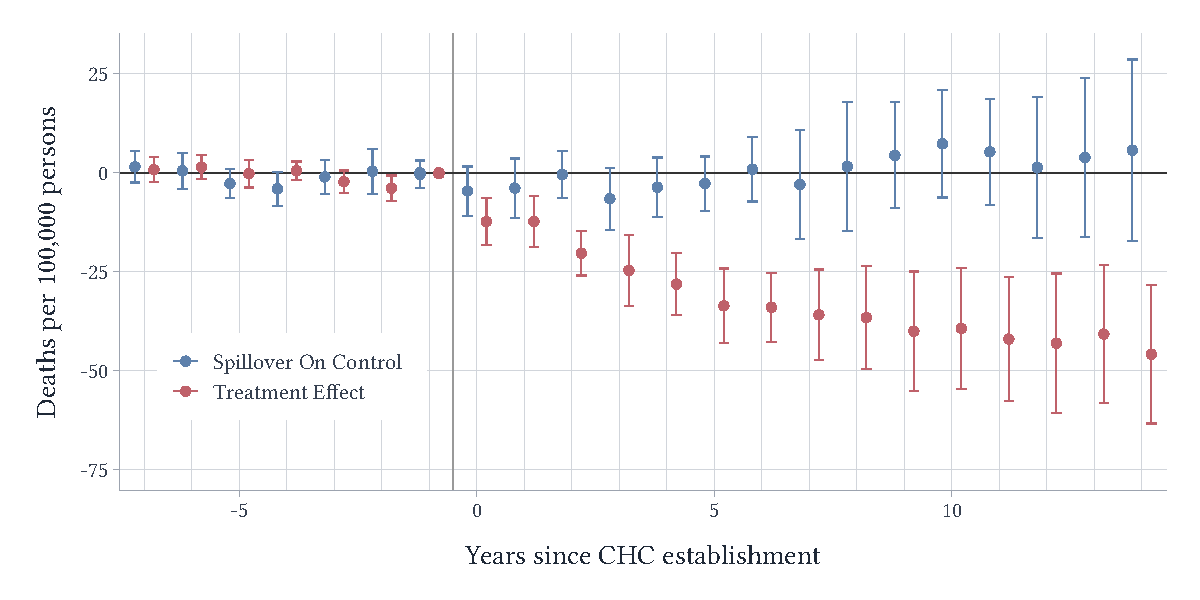
\includegraphics[width=\textwidth]{figures/spatial-spillovers/chc/chc-es_combined.pdf}
  }
  {\footnotesize
    \textit{Notes:} This figure plots event study estimates for the total effect and the spillover effect on control units within 25 miles of treatment at different periods relative to establishment year. The estimates are generated using the `did2s' package \citep{did2s}. 
  }
\end{figure}

There are theoretical reasons to think spillovers may or may not exist in this context. On the one hand, individuals outside the county can potentially travel to the community health centers to receive care. This would create a negative spillover effect on mortality rates in nearby counties which would bias their estimates towards zero. On the other hand, \citet{Bailey_Goodman_Bacon_2015} document evidence that their estimated effects are not due to emergencies but rather primary care services. In this case, it is less likely low-income individuals would travel very far to receive primary care, and hence the spillover effects are potentially near zero. My methodology can provide an answer to the question of how far do individuals travel for low-/no-cost primary care.

As in the method detailed above, I use an indicator for being within 25 miles of a treated county as the spillover variable. The results are presented in Figure \ref{fig:chc_es_spill}. The confidence intervals labeled with circles represent point estimates for the average spillover effect on control units within 25 miles. No spillover effect is estimated to be significantly different from zero which suggests that the effects of community health centers are very local. Since there are near zero spillover effects, the total effect estimates marked in Figure \ref{fig:chc_es_spill} as diamonds maintain the same shape as the author's original estimates with estimates between 15-30 fewer deaths per 100,000 persons. 

The spillover effects results provide evidence that low-income individuals will not travel far to receive primary care. Practically, this suggests that community health centers should be targeted to be as accessible as possible for poor individuals as they are unable to travel far to access the services. 

% ------------------------------------------------------------------------------
\section{Discussion}
\label{sec:conclusion}
% ------------------------------------------------------------------------------

This paper has considered the common environment where treatment is assigned to groups of units while the effects of treatment spread across these borders. I model this phenomenon using a potential outcomes framework and show why standard difference-in-differences estimation does not identify treatment effects of interest. Next, I discuss identification of two well-defined treatment effects. First, the average local effect of a single unit changing their treatment status is hard to identify without imposing assumptions on the spillover mapping. The second effect, the post-hoc average total effect on the treated is more simply identified under the assumption that spillovers are local. Effects can be identified by using far-away control units, but the practical usefullness of this result depends on whether far-away control units satisfy the parallel counterfactual trends. Last, I show how to extend the estimation strategy proposed in the paper to settings with staggered treatment-timing, a recent concern in the literature. 

I use a set of empirical examples to show that in settings with spatial spillovers, estimates can change significantly. In particular, place-based interventions change the nature of agglomeration in the local and surrounding area--that is cause spillovers--local effects of these policies can be misestimated without controlling for general equilibrium effects. I also show the importance of considering spillovers in weighing the pros and cons of various identification strategies. Identification strategies based on geographic continuity of unobservables can magnify the bias from spillovers as they restrict the comparison group to observations experiencing the largest spillover effects.



